
\section{The Algorithm}\label{sec:algo}

In this section, we present a simple version of the algorithm presented in \cite{Kel13}, called \texttt{SimpleSolver}. 

\begin{figure}[H]
\centering 
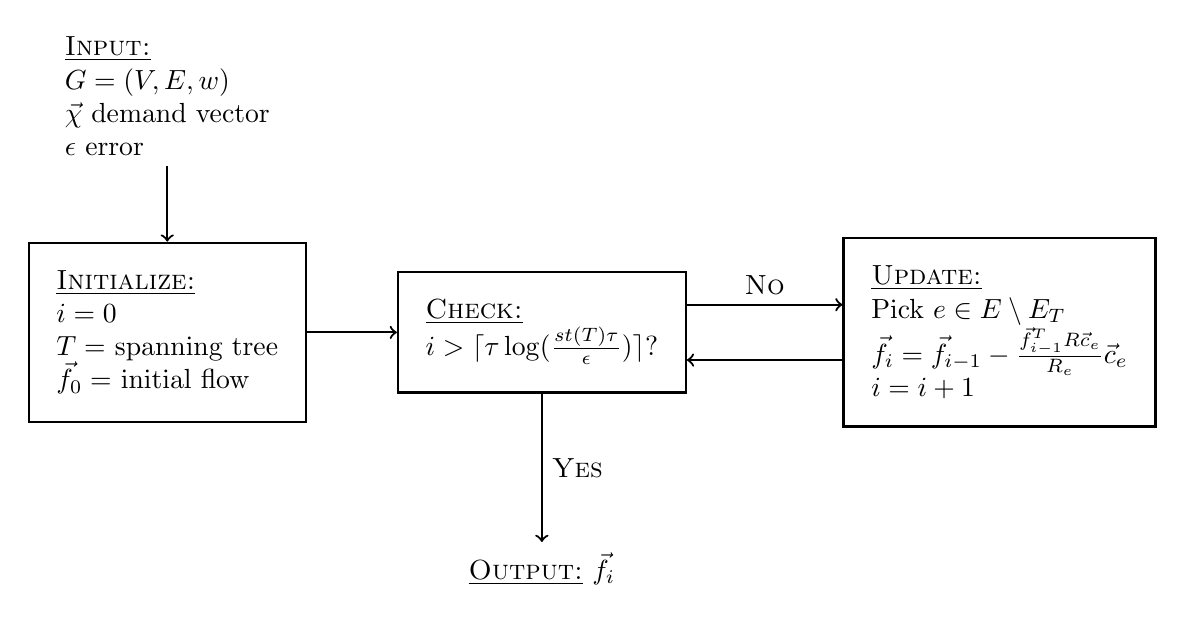
\begin{tikzpicture}[auto,node distance=3cm,align=left,
        thick,main node/.style={rectangle,draw,minimum size=1cm,inner sep=10pt]}]

    \node[] (1) {\underline{\textsc{Input:}}\\$G = (V,E,w)$\\ $\vec \chi$ demand vector \\ $\epsilon$ error};
    \node[main node] (2) [below of = 1]  {\underline{\textsc{Initialize:}}\\$i = 0$\\ $T = $ spanning tree \\$\vec f_0 = $ initial flow };
    \node[main node] (3) [xshift=5em, right of =2] {\underline{\textsc{Check:}}\\$i > \lceil \tau \log(\frac{st(T) \tau}{\epsilon} ) \rceil $?};
    \node[main node] (5) [xshift=8em, right of =3] {\underline{\textsc{Update:}} \\Pick $e \in E \setminus E_T$ \\$\vec f_i = \vec f_{i-1} - \frac{\vec f_{i-1}^T R \vec c_e}{R_e} \vec c_e $ \\ $i = i + 1$};
    \node[] (6) [below of=3] {\underline{\textsc{Output:}} $\vec f_i$};

    \path[->]
    (1) edge node {} (2)
    (2) edge node {} (3)
    (3) edge node {\textsc{Yes}} (6)
    (3) edge [transform canvas={yshift=1em}] node {\textsc{No}} (5)
    (5) edge  [transform canvas={yshift=-1em}] node {} (3);
\end{tikzpicture}
\caption{An outline of the \texttt{SimpleSolver} algorithm of \cite{Kel13} }
\end{figure}

\subsection{Initialization}
From Theorem \ref{thm:AN12}, the algorithm starts by choosing a spanning tree with stretch in $\mathcal O(m \log n \log \log n)$ in time $\mathcal O(m \log n \log \log n)$. 

An initial flow $\vec f_0$ is computed; this flow should be feasible, that is, satisfy $B^T\vec f = \vec \chi$. A feasible flow may be found in $\mathcal O(m + n)$ using Depth-First Search (DFS). Recalling that $\sum_{a \in V} \vec\chi (a) = 0$, we can make the reasonable simplifying assumption that, for some $s, t \in V$, $\vec \chi =  \textbf{1}_s - \textbf{1}_t$. $P_{(s,t)} \subseteq V \times V$ is the path between $s$ and $t$ in $T$. Now consider the flow $\vec f_0$ defined as $$ \vec f_0(a) = \begin{cases}
    1 & a \in P_{(s,t)} \\ 0 & \text{o.w.}
\end{cases}$$
By definition of the incidence matrix $B$, for each edge $e = (a,b) \in E$, the $e$th row of $B$ is $\textbf 1_{a}^T - \textbf 1_{b}^T$. So,  $$B^T \vec f_0 = \sum_{(a,b) \in P_{(s,t)}} \textbf 1_{a} - \textbf 1_{b} = \vec \chi,$$. which is feasible. So, a feasible initial flow $\vec f_0$ is computed in linear time using DFS. 

\subsection{Cycle Update}
\label{algorith:cycle-update}
In order to choose a cycle in the cycle basis, an edge is selected from $E \setminus E_T$. These edges are sampled with probability distribution $P(e) = \frac{1}{\tau(T)} \cdot \frac{R_e}{r_e}$. Once an edge $e$ is selected, the current flow $\vec f_{i-1}$ is updated:
$$\vec f_i = \vec f_{i-1} - \frac{\vec f_{i-1}^TR\vec c_e}{R_e}\vec c_e$$

The new flow satisfies KPL on the cycle $C_e$, that is: $\vec f_i^T R \vec c_e = 0$, since $\vec c_e^TR\vec c_e = R_e$. In addition, because $\vec c_e$ is a circulation, $B^T \vec c_e = 0$, which implies that the new flow is feasible, meaning $B^T \vec f_i = \vec \chi$. 

\subsection{Runtime}

Initialization runs in $\mathcal O(m \log n \log \log n)$. Cycle updates, which are repeated $\lceil \tau \log (\frac{st(T) \tau}{\epsilon}) \rceil$ times, can be performed in $\mathcal O(\log n)$, using a data structure presented in \cite{Kel13} which is out of scope of these lecture notes. In all, algorithm runs in $\mathcal O (m \log^2 n \log{ \log n \log{(\epsilon^{{-1}})}})$. 

% \begin{algorithm}
% \SetAlgoLined
% \SetKwInOut{Input}{Input}
% \SetKwInOut{Output}{Output}
% \Input{$G = (V, E, r)$, $\boundary \in \rvertvec$, $\epsilon \in \rPos$}
% \Output{$\flow \in \redgevec$ and $\volt \in \rvertvec$}
% \BlankLine
% \ \ $T := $ low-stretch spanning tree of $G$\;\\
% $\flow_0 := $ unique flow on $T$ such that $\incMatrix^T \flow_0 = \boundary$\;\\
% $\edgeSampleProb{e} := \frac{1}{\treeCondition(\tree)} \cdot \frac{\cycleResistance{e}}{r_e}$ for all
% $e \in \offtreeEdgeSet$ \;\\
% $\nIter = \big\lceil\treeCondition \log \big(\frac{\stretchTotal{\tree}
%     \cdot \treeCondition(\tree)}{\epsilon}\big)\big\rceil$\;\\
% \For{$i = 1$ to $\nIter$}
% {
%     Pick random $e_i \in \offtreeEdgeSet$ by probability distribution
%     $\sampleProbVec$ \;\\ 
%     $\flow_i = \flow_{i - 1} - \frac{\cyclePotential{e}{\flow_{i - 1}}}
%         {\cycleResistance{e}}
%     \treeCycleVec{e}$ \;
% }
% \Return{$\flow_{\nIter}$ and its tree induced voltages $\volt_{\nIter}$}
% \caption{\label{algm:simplealgorithm}$\simpleSolver$}
% \end{algorithm}